%% %% %% %%
%%
%% Parte B de la práctica
%%
%% %% %% %%

\documentclass[../procedimientos.tex]{subfiles}
\graphicspath{{\subfix{../../images/}}}

\begin{document}
\clearpage
\subsection{Parte B}
\subsubsection{Instrucciones}
Diseñar e implementar un circuito digital que mediante una señal de control 
$C$ pueda seleccionar el tipo de conversión de código: con $C=1$, GRAY a 
BINARIO y con $C=0$, BINARIO a GRAY. El código es de tres bits.
\begin{figure}[H]
  \centering
  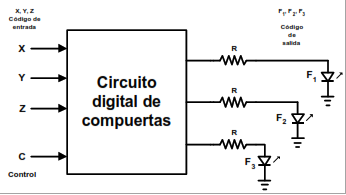
\includegraphics[width=0.5\textwidth]{b_instruction}
  \caption{Ejercicio B}
  \label{fig:b_inst}
\end{figure}

\subsubsection{Análisis}
Primero, es importante plantear la tabla de verdad del problema. Para este 
caso, se tienen  tres entradas: $c$, $x$, $y$ y $z$. De los anteriores, para 
la representación de 3 bits del número, únicamente se consideran $x$, $y$ y 
$z$; mientras qeu $c$ únicamente se considera como una bandera. Por otra 
parte, la salida está compuesta de tres bits: $f_1$ (bit más signiticativo), 
$f_2$ y $f_3$ (bit menos signifivativo).

\begin{table}[H]
  \centering
  \begin{tabular}{cccc|ccc}
    \hline
    $c$ & $x$ & $y$ & $z$ & $f_1$ & $f_2$ & $f_3$\\
    \hline
    0 & 0 & 0 & 0 & 0 & 0 & 0\\
    0 & 0 & 0 & 1 & 0 & 0 & 1\\
    0 & 0 & 1 & 0 & 0 & 1 & 1\\
    0 & 0 & 1 & 1 & 0 & 1 & 0\\
    0 & 1 & 0 & 0 & 1 & 1 & 0\\
    0 & 1 & 0 & 1 & 1 & 1 & 1\\
    0 & 1 & 1 & 0 & 1 & 0 & 1\\
    0 & 1 & 1 & 1 & 1 & 0 & 0\\
    1 & 0 & 0 & 0 & 0 & 0 & 0\\
    1 & 0 & 0 & 1 & 0 & 0 & 1\\
    1 & 0 & 1 & 1 & 0 & 1 & 1\\
    1 & 0 & 1 & 0 & 0 & 1 & 0\\
    1 & 1 & 1 & 0 & 1 & 1 & 1\\
    1 & 1 & 1 & 1 & 1 & 1 & 0\\
    1 & 1 & 0 & 1 & 1 & 0 & 0\\
    1 & 1 & 0 & 0 & 1 & 0 & 1\\
    \hline
  \end{tabular}
  \caption{Tabla de verdad del problema (Sección A)}
  \label{tab:tv_a}
\end{table}

La tabla de verdad descrita anteriormente, se describe el comportamiento de 
tres funciones lógicas: $f_1(cxyz)$, $f_2(cxyz)$ y $f_3(cxyz)$. Para deducir 
los circuitos a utilizar, se utilizará la forma canónica \textit{SOP} y a 
través de una reducción se simplificará la expresión, tal como se muestra a 
continuación.

Para $f_1(cxyz)$, se tiene la siguiente forma canónica:
\begin{equation*}
  f_1(cxyz) = \sum_m (4, 5, 6, 7, 12, 13, 14, 15)
\end{equation*}

Desarrollando la expresión:
\begin{align*}
  f_1(cxyz) &= \nt{c}x\nt{y}\nt{z} + \nt{c}x\nt{y}z + \nt{c}xy\nt{z} + 
  \nt{c}xyz + cx\nt{y}\nt{z} + cx\nt{y}z + cxy\nt{z} + cxyz\\
  &= x(\nt{c}\nt{y}\nt{z} + \nt{c}\nt{y}z + \nt{c}y\nt{z} + \nt{c}yz + 
  c\nt{y}\nt{z} + c\nt{y}z + cy\nt{z} + cyz)\\
  &= x(1)\\
  &= x
\end{align*}
\begin{equation*}
  \boxed{
    \therefore f_1(cxyz) = x
  }
\end{equation*}

Continuando con el cálculo de $f_2(cxyz)$, se tiene la siguiente forma 
canónica:
\begin{equation*}
  f_2(cxyz) = \sum_m (2, 3, 4, 5, 10, 11, 12, 13)
\end{equation*}

Desarrollando la expresión:
\begin{align*}
  f_2(cxyz) &= \nt{c}\nt{x}y\nt{z} + \nt{c}\nt{x}yz + \nt{c}x\nt{y}\nt{z} + 
  \nt{c}x\nt{y}z + c\nt{x}y\nt{z} + c\nt{x}yz + cx\nt{y}\nt{z} + cx\nt{y}z\\
  &= (\nt{c}\nt{x}y\nt{z} + \nt{c}\nt{x}yz) + (\nt{c}x\nt{y}\nt{z} + 
  \nt{c}x\nt{y}z) + (c\nt{x}y\nt{z} + c\nt{x}yz) + (cx\nt{y}\nt{z} + 
  cx\nt{y}z)\\
  &= \nt{c}\nt{x}y + \nt{c}x\nt{y} + c\nt{x}y + cx\nt{y}\\
  &= (\nt{c}\nt{x}y + c\nt{x}y) + (\nt{c}x\nt{y} + cx\nt{y})\\
  &= \nt{x}y + x\nt{y}\\
  &= x \oplus y
\end{align*}
\begin{equation*}
  \boxed{
    \therefore f_2(cxyz) = x \oplus y
  }
\end{equation*}

Finalmente, continuando con el cálculo de $f_3(cxyz)$, se tiene la siguiente 
forma canónica:
\begin{equation*}
  f_3(cxyz) = \sum_m (1, 2, 5, 6, 9, 10, 12, 15)
\end{equation*}

Desarrollando la expresión:
\begin{align*}
  f_3(cxyz) &= \nt{c}\nt{x}\nt{y}z + \nt{c}\nt{x}y\nt{z} + \nt{c}x\nt{y}z + 
  \nt{c}xy\nt{z} + c\nt{x}\nt{y}z + c\nt{x}y\nt{z} + cx\nt{y}\nt{z} + cxyz\\
  &= (\nt{c}\nt{x}\nt{y}z + c\nt{x}\nt{y}z) + (\nt{c}\nt{x}y\nt{z} + 
  c\nt{x}y\nt{z}) + (\nt{c}x\nt{y}z + \nt{c}xy\nt{z} + cx\nt{y}\nt{z} + 
  cxyz)\\
  &= \nt{x}\nt{y}z + \nt{x}y\nt{z} + x(\nt{c}\nt{y}z + \nt{c}y\nt{z} + 
  c\nt{y}\nt{z} + cyz)\\
  &= \nt{x}(\nt{y}z + y\nt{z}) + x(\nt{c}(\nt{y}z + y\nt{z}) + c(\nt{y}\nt{z} 
  + yz))\\
  &= \nt{x}(y \oplus z) + x(\nt{c}(y \oplus z) + c(y \odot z))\\
  &= \nt{x}(y \oplus z) + x(c \oplus (y \oplus z))
\end{align*}
\begin{equation*}
  \boxed{
    \therefore f_3(cxyz) = \nt{x}(y \oplus z) + x(c \oplus (y \oplus z))
  }
\end{equation*}


\subsubsection{Implementación en Quartus}

\end{document}

